\begin{figure}[H]
\centering
\caption{Fluxo de eventos RFID suportado pela arquitetura}
\resizebox{0.94\textwidth}{!}{
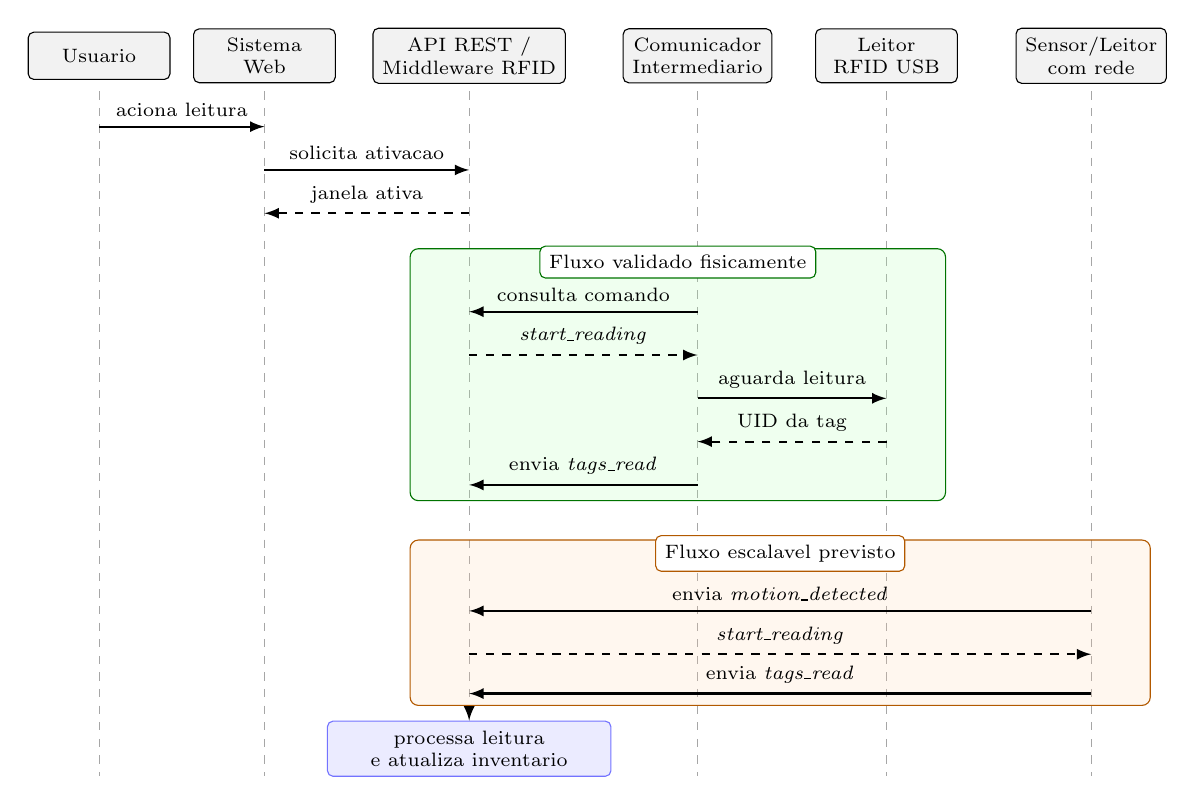
\begin{tikzpicture}[
    font=\scriptsize,
    participant/.style={draw, rounded corners=2pt, align=center, minimum width=1.8cm, minimum height=0.6cm, fill=gray!10},
    msg/.style={->, >=latex, thick},
    reply/.style={->, >=latex, thick, dashed},
    lifeline/.style={dashed, gray!70},
    altbox/.style={draw, rounded corners=3pt, fill opacity=0.18, text opacity=1},
    labelbox/.style={draw, rounded corners=2pt, fill=white, align=center, font=\scriptsize},
    process/.style={draw, rounded corners=2pt, align=center, fill=blue!8, draw=blue!55, minimum width=3.6cm, minimum height=0.7cm}
]

\def\top{0}
\def\bottom{-9.15}

% Participantes principais
\node[participant] (u) at (0,\top) {Usuario};
\node[participant] (web) at (2.1,\top) {Sistema\\Web};
\node[participant] (api) at (4.7,\top) {API REST /\\Middleware RFID};
\node[participant] (gw) at (7.6,\top) {Comunicador\\Intermediario};
\node[participant] (usb) at (10.0,\top) {Leitor\\RFID USB};
\node[participant] (rede) at (12.6,\top) {Sensor/Leitor\\com rede};

\foreach \x in {0,2.1,4.7,7.6,10.0,12.6}
  \draw[lifeline] (\x,-0.45) -- (\x,\bottom);

% Acionamento inicial pelo sistema web
\draw[msg] (0,-0.9) -- node[above]{aciona leitura} (2.1,-0.9);
\draw[msg] (2.1,-1.45) -- node[above]{solicita ativacao} (4.7,-1.45);
\draw[reply] (4.7,-2.0) -- node[above]{janela ativa} (2.1,-2.0);

% Fluxo validado fisicamente
\draw[altbox, fill=green!35, draw=green!45!black] (3.95,-2.45) rectangle (10.75,-5.65);
\node[labelbox, draw=green!45!black] at (7.35,-2.62) {Fluxo validado fisicamente};
\draw[msg] (7.6,-3.25) -- node[above]{consulta comando} (4.7,-3.25);
\draw[reply] (4.7,-3.8) -- node[above]{\textit{start\_reading}} (7.6,-3.8);
\draw[msg] (7.6,-4.35) -- node[above]{aguarda leitura} (10.0,-4.35);
\draw[reply] (10.0,-4.9) -- node[above]{UID da tag} (7.6,-4.9);
\draw[msg] (7.6,-5.45) -- node[above]{envia \textit{tags\_read}} (4.7,-5.45);

% Fluxo escalavel previsto
\draw[altbox, fill=orange!35, draw=orange!70!black] (3.95,-6.15) rectangle (13.35,-8.25);
\node[labelbox, draw=orange!70!black] at (8.65,-6.32) {Fluxo escalavel previsto};
\draw[msg] (12.6,-7.05) -- node[above]{envia \textit{motion\_detected}} (4.7,-7.05);
\draw[reply] (4.7,-7.6) -- node[above]{\textit{start\_reading}} (12.6,-7.6);
\draw[msg] (12.6,-8.1) -- node[above]{envia \textit{tags\_read}} (4.7,-8.1);

% Processamento comum
\node[process] (proc) at (4.7,-8.8) {processa leitura\\e atualiza inventario};
\draw[msg] (4.7,-8.3) -- (proc.north);

\end{tikzpicture}
}
\vspace{0.3em}
\legend{Fonte: Elaborado pelo autor (2026).}
\label{fig:fluxo-eventos-rfid}
\end{figure}
